\renewcommand{\thefigure}{\Asbuk{section}.\arabic{figure}}
\renewcommand{\thetable}{\Asbuk{section}.\arabic{table}}
\renewcommand{\thelstlisting}{\Asbuk{section}.\arabic{lstlisting}}

\chapter*{Приложение А}
\addcontentsline{toc}{chapter}{Приложение А}

\setcounter{section}{1}
\setcounter{figure}{0}
\setcounter{table}{0}
\setcounter{lstlisting}{0}

На приведенных ниже рисунках показана зависимость разности
величин~\eqref{eq:dst_param},
полученных классической линейной регрессией и методом симметричной аппроксимации,
от с.к.о. ошибок наблюдений \( \sigma_{\varepsilon_x}, \sigma_{\varepsilon_y} \) при
различных фактических значениях коэффициента усиления \( beta \)
линейной стохастической системы второго типа.

\begin{figure}[h]
  \centering
  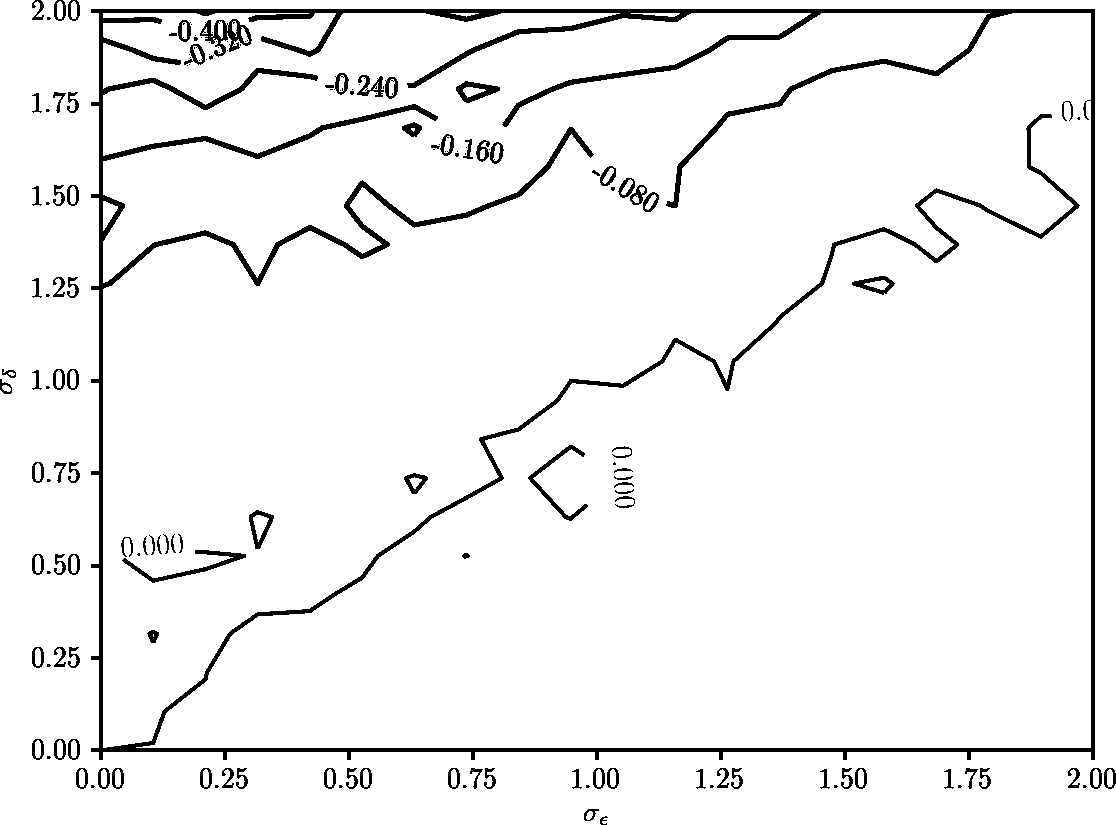
\includegraphics[width=150mm]{fig/linear/param/beta-0,125_param.png}
  \caption{Точность оценивания параметров модели при \( \beta = 0{,}125 \)}
\end{figure}

\begin{figure}[h]
  \centering
  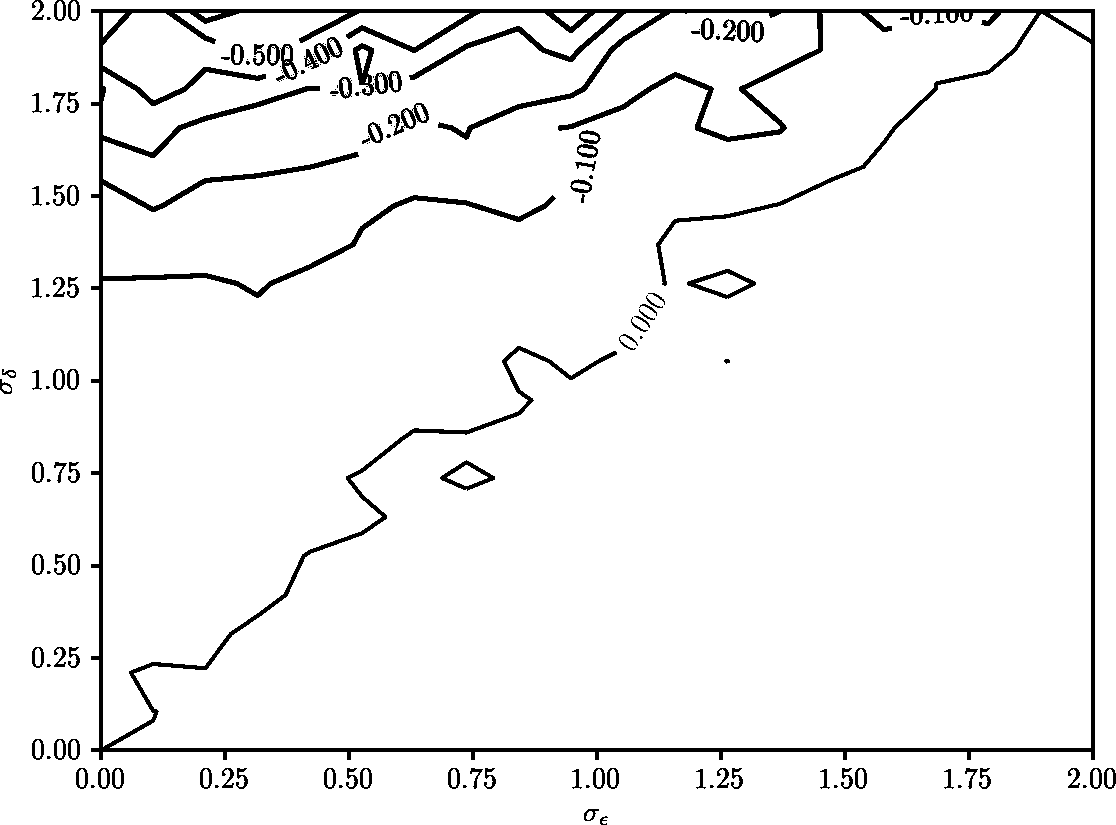
\includegraphics[width=150mm]{fig/linear/param/beta-0,2_param.png}
  \caption{Точность оценивания параметров модели при \( \beta = 0{,}2 \)}
\end{figure}

\begin{figure}[h]
  \centering
  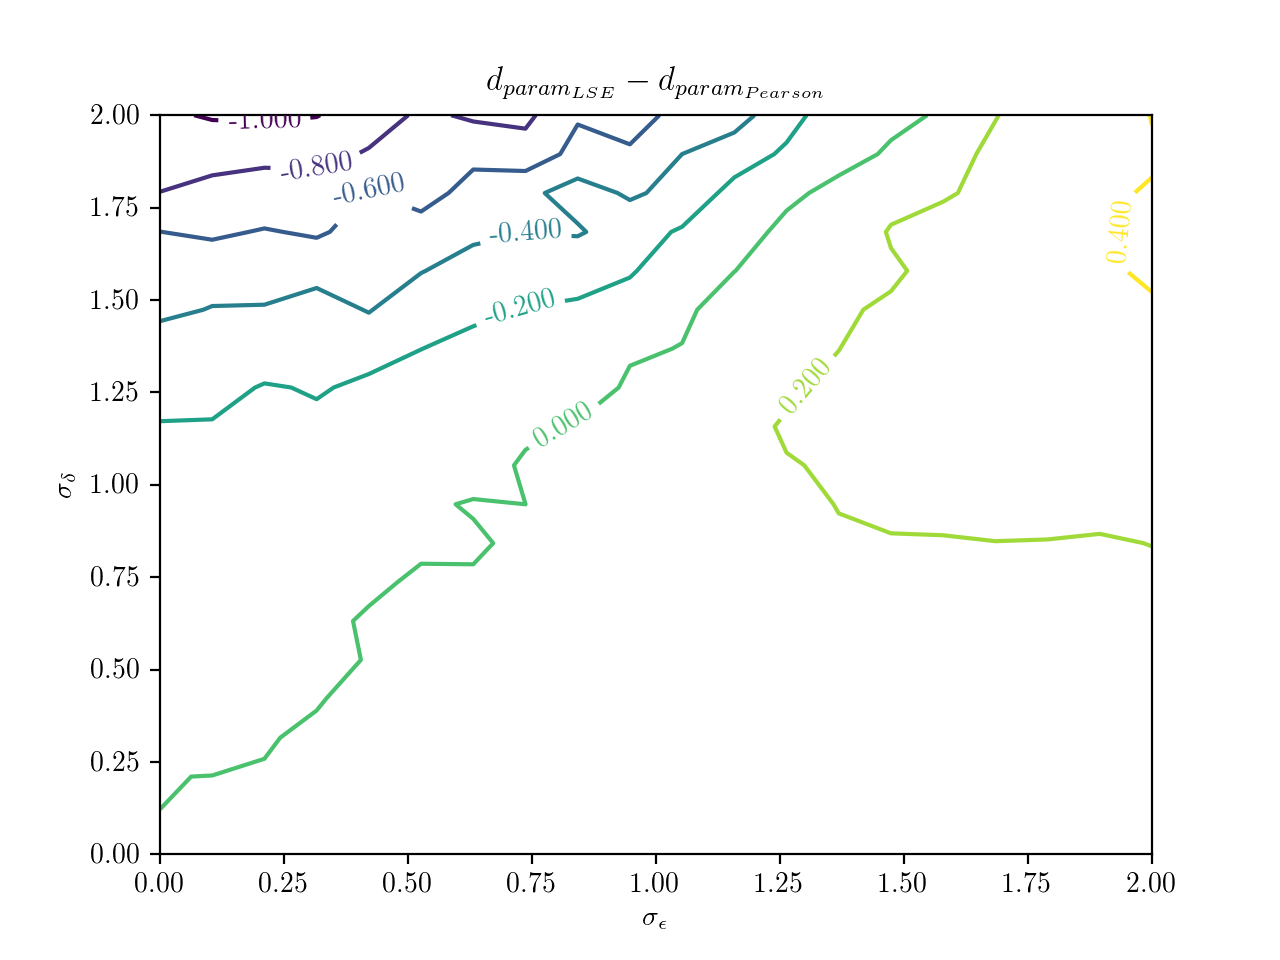
\includegraphics[width=150mm]{fig/linear/param/beta-0,5_param.png}
  \caption{Точность оценивания параметров модели при \( \beta = 0{,}5 \)}
\end{figure}

\begin{figure}[h]
  \centering
  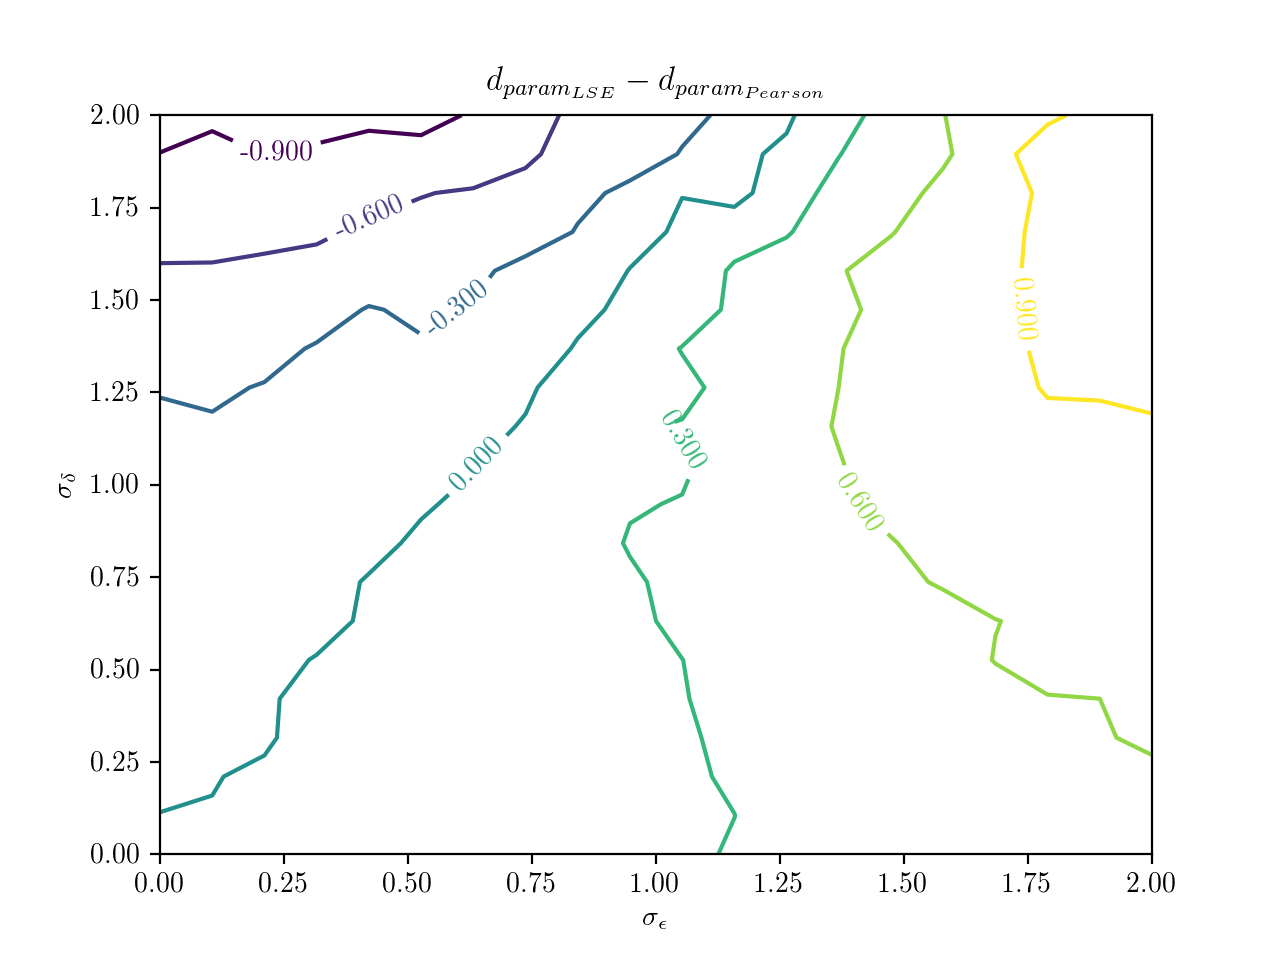
\includegraphics[width=150mm]{fig/linear/param/beta-1_param.png}
  \caption{Точность оценивания параметров модели при \( \beta = 1\)}
\end{figure}

\begin{figure}[h]
  \centering
  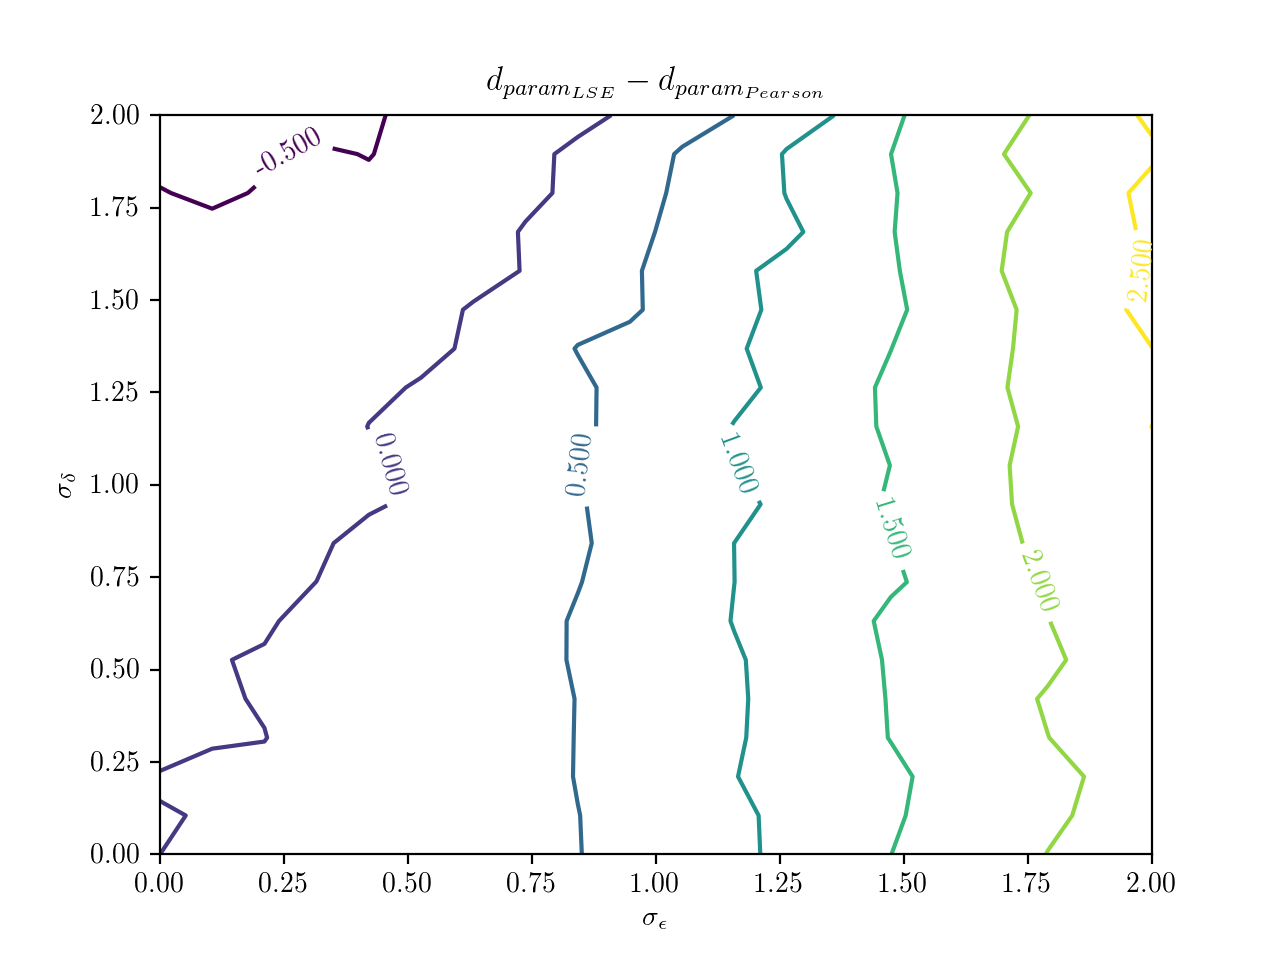
\includegraphics[width=150mm]{fig/linear/param/beta-2_param.png}
  \caption{Точность оценивания параметров модели при \( \beta = 2 \)}
\end{figure}

\begin{figure}[h]
  \centering
  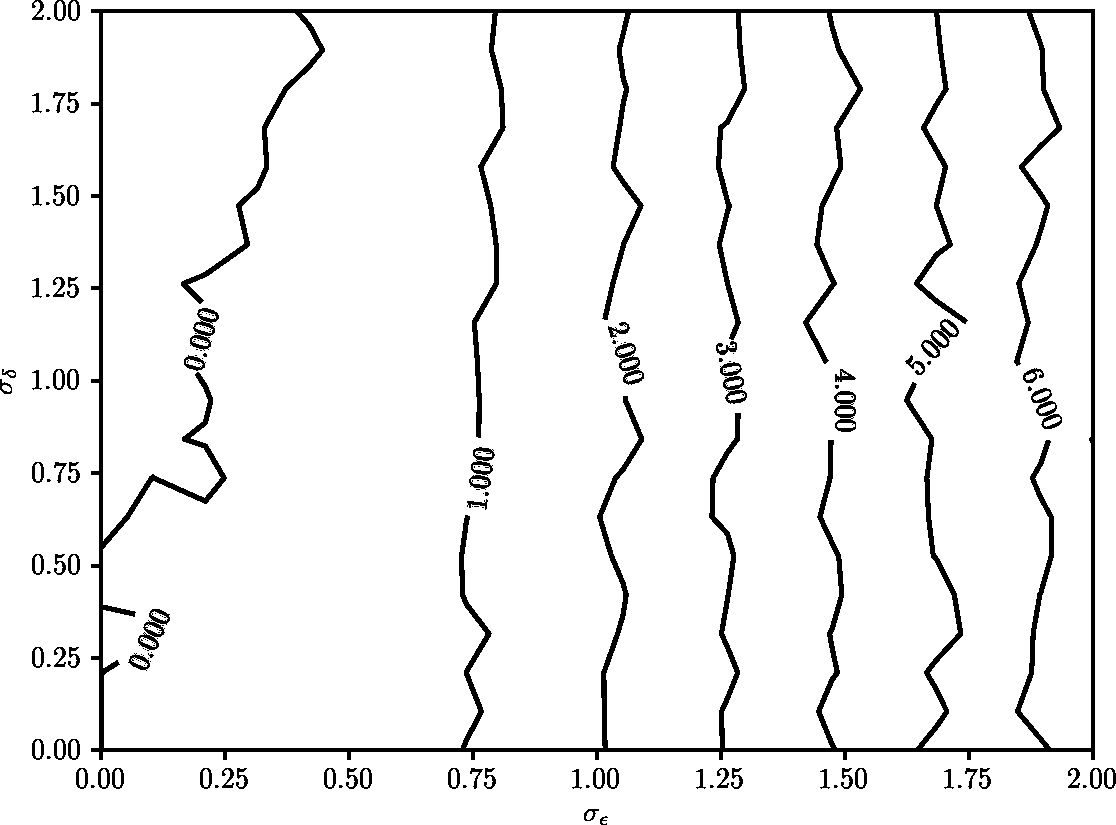
\includegraphics[width=150mm]{fig/linear/param/beta-5_param.png}
  \caption{Точность оценивания параметров модели при \( \beta = 5 \)}
\end{figure}

\begin{figure}[h]
  \centering
  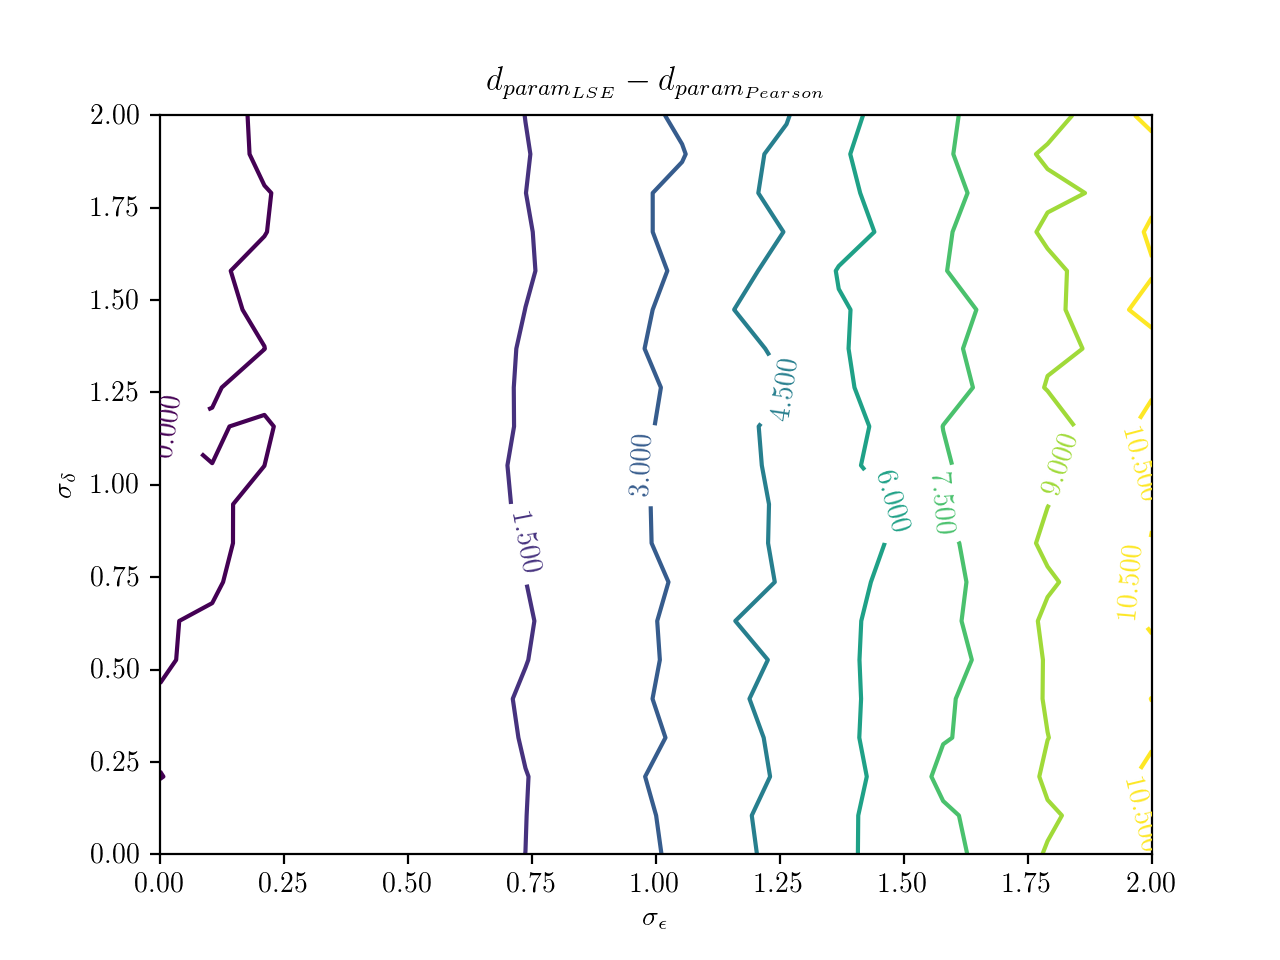
\includegraphics[width=150mm]{fig/linear/param/beta-8_param.png}
  \caption{Точность оценивания параметров модели при \( \beta = 8 \)}
\end{figure}
